\documentclass[TC, exos, e,p]{phBook}
\def\urlcorrection{https://phlered.github.io/depot_github/TCO/exercice_supp_correction.pdf}
%Options : 2, 1, T, SNT (classes), p, b,prof, exos, cours, DS, noir, a4, a5, twocolumn, landscape

\begin{document}
\setcounter{chapter}{6} %Numéro du chapitre précédent
\chapter{Exercices supplémentaires : lois discrètes}
%%%%%%%%%%%%%%%%%%%%%%%%


\begin{exercice}
    \begin{enonce}
        Dans cet exercice, les réponses seront arrondies à $10^{-3}$ près.

Une entreprise fabrique des composants électroniques. Pour améliorer la qualité de sa production, elle a mis en place un système de contrôle qualité.

On sait que $5\,\%$ des composants produits sont défectueux. Parmi les composants défectueux, $95\,\%$ sont détectés par le système de contrôle. Parmi les composants non défectueux, $3\,\%$ sont signalés comme défectueux par le système.

\bigskip

On choisit un composant au hasard dans la production. On note les évènements suivants :

\begin{description}
\item[ ] $D$ : \og le composant est défectueux\fg{}
\item[ ] $S$ : \og le composant est signalé défectueux par le système\fg{}.
\end{description}

Les évènements contraires des évènements $D$ et $S$ sont notés respectivement $\overline{D}$ et $\overline{S}$.

\bigskip

\textbf{Partie A : Probabilités conditionnelles}

\begin{enumerate}
\item À partir de l'énoncé, donner, sans calcul, les probabilités $P(D)$ et les probabilités conditionnelles $P_D(S)$ et $P_{\overline{D}}(S)$.

\item
	\begin{enumerate}
		\item Calculer $P(D \cap S)$.
		\item En déduire $P\left(\overline{D} \cap S\right)$.
	\end{enumerate}

\item Recopier l'arbre des probabilités ci-dessous et le compléter.

\begin{center}
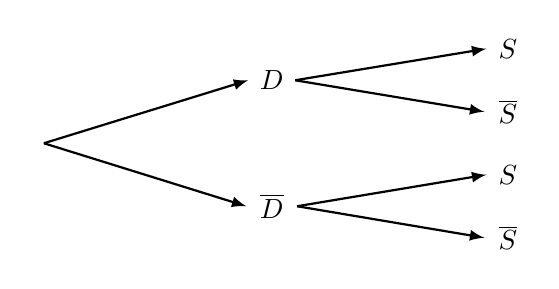
\begin{tikzpicture}[xscale=1,yscale=1,baseline={(R.base)}]
% Styles
\tikzstyle{fleche}=[->,>=latex,thick]
\tikzstyle{noeud}=[fill=white,circle,inner sep=2pt]
\tikzstyle{feuille}=[fill=white,circle,inner sep=2pt]
\tikzstyle{etiquette}=[pos=0.6,fill=white, inner xsep=3pt, inner ysep=1.5pt]
% Dimensions
\def\DistanceInterNiveaux{3}
\def\DistanceInterFeuilles{0.8}
% Dimensions calculées
\def\NiveauA{(0)*\DistanceInterNiveaux}
\def\NiveauB{(1)*\DistanceInterNiveaux}
\def\NiveauC{(2)*\DistanceInterNiveaux}
\def\InterFeuilles{(-1)*\DistanceInterFeuilles}
% Noeuds
\node[noeud] (R) at ({\NiveauA},{(1.5)*\InterFeuilles}) {};
\node[noeud] (Ra) at ({\NiveauB},{(0.5)*\InterFeuilles}) {$D$};
\node[feuille] (Raa) at ({\NiveauC},{(0)*\InterFeuilles}) {$S$};
\node[feuille] (Rab) at ({\NiveauC},{(1)*\InterFeuilles}) {$\overline{S}$};
\node[noeud] (Rb) at ({\NiveauB},{(2.5)*\InterFeuilles}) {$\overline{D}$};
\node[feuille] (Rba) at ({\NiveauC},{(2)*\InterFeuilles}) {$S$};
\node[feuille] (Rbb) at ({\NiveauC},{(3)*\InterFeuilles}) {$\overline{S}$};
% Arcs
\draw[fleche] (R.east)--(Ra.west);% node[etiquette] {$$};
\draw[fleche] (Ra.east)--(Raa.west);% node[etiquette] {$$};
\draw[fleche] (Ra.east)--(Rab.west);% node[etiquette] {$$};
\draw[fleche] (R.east)--(Rb.west);% node[etiquette] {$$};
\draw[fleche] (Rb.east)--(Rba.west);% node[etiquette] {$$};
\draw[fleche] (Rb.east)--(Rbb.west);% node[etiquette] {$$};
\end{tikzpicture}
\end{center}

\item Calculer $P(S)$ et interpréter le résultat dans le contexte de l'exercice.

\item Un composant est signalé défectueux par le système. Quelle est la probabilité qu'il soit réellement défectueux ? Interpréter ce résultat.
\end{enumerate}

\bigskip

\textbf{Partie B : Loi binomiale}

On prélève un échantillon de $30$ composants au hasard dans la production. La production est suffisamment importante pour qu'on puisse assimiler ce choix à des tirages successifs avec remise.

On note $X$ la variable aléatoire qui compte le nombre de composants défectueux dans cet échantillon.

\emph{On rappelle que, pour un composant choisi au hasard, la probabilité qu'il soit défectueux est} $p = 0,05$.

\begin{enumerate}[resume]
\item
	\begin{enumerate}
		\item Justifier que $X$ suit une loi binomiale dont on précisera les paramètres.
		\item Calculer, en rappelant la formule, la probabilité qu'il y ait exactement $2$ composants défectueux dans cet échantillon.
		\item Calculer la probabilité qu'il y ait au plus $3$ composants défectueux.
		\item Calculer la probabilité qu'il y ait au moins $2$ composants défectueux.
	\end{enumerate}

\item On souhaite déterminer la taille minimale $n$ d'un échantillon pour que la probabilité d'observer au moins un composant défectueux soit supérieure à $0,95$.
	\begin{enumerate}
		\item Exprimer la probabilité de l'évènement \og l'échantillon contient au moins un composant défectueux\fg{} en fonction de $n$.
		\item En déduire une inéquation que doit vérifier $n$.
		\item Résoudre cette inéquation% avec l'aide du logarithme népérien
		et déterminer la valeur minimale de $n$.
	\end{enumerate}
\end{enumerate}

    \end{enonce}
    %%%%%%%%%%%

    \begin{correction}
        \textbf{Partie A : Probabilités conditionnelles}

\begin{enumerate}
\item D'après l'énoncé :
\begin{itemize}
\item $P(D) = 0,05$, car 5~\% des composants produits sont défectueux;
\item $P_D(S) = 0,95$, car 95~\% des composants défectueux sont détectés par le système;
\item $P_{\overline{D}}(S) = 0,03$, car 3~\% des composants non défectueux sont incorrectement signalés.
\end{itemize}

\item 
	\begin{enumerate}
		\item On a :\quad $P(D \cap S) = P(D) \times P_D(S) = 0,05 \times 0,95 = 0,0475$.
		\item D'après la formule des probabilités totales :

$P(S) = P(D \cap S) + P\big(\,\overline{D}\cap S\big)$

D'où : \quad $P\big(\,\overline{D} \cap S\big) = P(S) - P(D \cap S)$

On a aussi : $P\big(\,\overline{D} \cap S\big) = P\big(\,\overline{D}\,\big) \times P_{\overline{D}}(S) = 0,95 \times 0,03 = 0,0285$
	\end{enumerate}

\item Voici l'arbre de probabilités complété :

\begin{center}
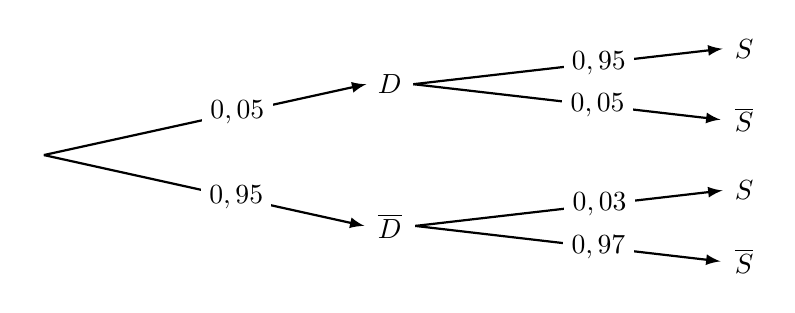
\begin{tikzpicture}[xscale=1,yscale=1,baseline={(R.base)}]
% Styles
\tikzstyle{fleche}=[->,>=latex,thick]
\tikzstyle{noeud}=[fill=white,circle,inner sep=2pt]
\tikzstyle{feuille}=[fill=white,circle,inner sep=2pt]
\tikzstyle{etiquette}=[pos=0.6,fill=white, inner xsep=3pt, inner ysep=1.5pt]
% Dimensions
\def\DistanceInterNiveaux{4.5}
\def\DistanceInterFeuilles{0.9}
% Dimensions calculées
\def\NiveauA{(0)*\DistanceInterNiveaux}
\def\NiveauB{(1)*\DistanceInterNiveaux}
\def\NiveauC{(2)*\DistanceInterNiveaux}
\def\InterFeuilles{(-1)*\DistanceInterFeuilles}
% Noeuds
\node[noeud] (R) at ({\NiveauA},{(1.5)*\InterFeuilles}) {};
\node[noeud] (Ra) at ({\NiveauB},{(0.5)*\InterFeuilles}) {$D$};
\node[feuille] (Raa) at ({\NiveauC},{(0)*\InterFeuilles}) {$S$};
\node[feuille] (Rab) at ({\NiveauC},{(1)*\InterFeuilles}) {$\overline{S}$};
\node[noeud] (Rb) at ({\NiveauB},{(2.5)*\InterFeuilles}) {$\overline{D}$};
\node[feuille] (Rba) at ({\NiveauC},{(2)*\InterFeuilles}) {$S$};
\node[feuille] (Rbb) at ({\NiveauC},{(3)*\InterFeuilles}) {$\overline{S}$};
% Arcs
\draw[fleche] (R.east)--(Ra.west) node[etiquette] {$0,05$};
\draw[fleche] (Ra.east)--(Raa.west) node[etiquette] {$0,95$};
\draw[fleche] (Ra.east)--(Rab.west) node[etiquette] {$0,05$};
\draw[fleche] (R.east)--(Rb.west) node[etiquette] {$0,95$};
\draw[fleche] (Rb.east)--(Rba.west) node[etiquette] {$0,03$};
\draw[fleche] (Rb.east)--(Rbb.west) node[etiquette] {$0,97$};
\end{tikzpicture}
\end{center}

\item D'après la formule des probabilités totales :

$P(S) = P(D \cap S) + P\big(\,\overline{D} \cap S\big) = 0,0475 + 0,0285 = 0,076$

Dans le contexte de l'exercice, cela signifie qu'environ 7,6~\% des composants sont signalés comme défectueux par le système de contrôle.

\item On cherche $P_S(D)$ :

$P_S(D) = \dfrac{P(S \cap D)}{P(S)} = \dfrac{0,0475}{0,076} \approx 0,625$

Dans le contexte de l'exercice, cela signifie que lorsqu'un composant est signalé défectueux par le système, il y a environ 62,5~\% de chances qu'il soit réellement défectueux.
\end{enumerate}

\bigskip

\textbf{Partie B : Loi binomiale}

\begin{enumerate}[resume]
\item
	\begin{enumerate}
		\item 
\begin{itemize}
\item On a une épreuve aléatoire à deux issues. On qualifie de succès l'évènement $D$, de probabilité $p = 0,05$;
\item Cette épreuve est répétée $n =30$ fois pour constituer l'échantillon de 30 composants. La répétition étant assimilable à des tirages successifs avec remise, les répétitions sont identiques et indépendantes;
\item La variable aléatoire $X$ compte le nombre de composants défectueux, donc le nombre de succès, dans l'échantillon.
\end{itemize}

Ces trois éléments garantissent que $X$ suit la loi binomiale, de paramètres $n = 30$ et $p = 0,05$.

		\item La probabilité qu'il y ait exactement 2 composants défectueux est :

$P(X = 2) = \displaystyle \binom{30}{2}\times 0,05^2 \times 0,95^{28} = 435 \times 0,05^2 \times 0,95^{28} \approx 0,259$

		\item La probabilité qu'il y ait au plus 3 composants défectueux est :

$P(X \le 3) = P(X = 0) + P(X = 1) + P(X = 2) + P(X = 3)$

$P(X \le 3) = \displaystyle \binom{30}{0}\times 0,95^{30} + \binom{30}{1}\times 0,05 \times 0,95^{29} + \binom{30}{2}\times 0,05^2 \times 0,95^{28} + \binom{30}{3}\times 0,05^3 \times 0,95^{27}$

$P(X \le 3) \approx 0,939$

		\item La probabilité qu'il y ait au moins 2 composants défectueux est :

$P(X \ge 2) = 1 - P(X < 2) = 1 - P(X = 0) - P(X = 1)$

$P(X \ge 2) = 1 - 0,95^{30} - 30 \times 0,05 \times 0,95^{29}$

$P(X \ge 2) \approx 1 - 0,215 - 0,339 \approx 0,446$
	\end{enumerate}

\item
	\begin{enumerate}
		\item Soit $Y$ la variable aléatoire qui compte le nombre de composants défectueux dans un échantillon de taille $n$. Alors $Y$ suit une loi binomiale de paramètres $n$ et $p = 0,05$.

La probabilité de l'évènement \og l'échantillon contient au moins un composant défectueux\fg{} est :

$P(Y \ge 1) = 1 - P(Y = 0) = 1 - 0,95^n$

		\item On cherche $n$ tel que :

$1 - 0,95^n > 0,95 \iff 0,95^n < 0,05$

		\item On résout l'inéquation $0,95^n < 0,05$ :

\begin{align*}
0,95^n &< 0,05 \\
\ln\left(0,95^n\right) &< \ln(0,05) \quad \text{(car $\ln$ est strictement croissante)} \\
n \ln(0,95) &< \ln(0,05) \\
n &> \dfrac{\ln(0,05)}{\ln(0,95)} \quad \text{(on change le sens car $\ln(0,95) < 0$)}
\end{align*}

On calcule : $\dfrac{\ln(0,05)}{\ln(0,95)} \approx \dfrac{-2,996}{-0,051} \approx 58,4$

La valeur minimale de $n$ est donc $\boxed{n = 59}$.
	\end{enumerate}
\end{enumerate}

    \end{correction}
\end{exercice}
%%%%%%%%%%%%%%%%%%%%%
%%% Fin exercice %%%%
%%%%%%%%%%%%%%%%%%%%%









\begin{exercice}
    \begin{enonce}
        Une machine industrielle est équipée d'un composant qui peut tomber en panne. On suppose que chaque jour, indépendamment des jours précédents, la probabilité que ce composant tombe en panne est de $0,08$.

On note $X$ la variable aléatoire égale au nombre de jours nécessaires pour observer la première panne du composant.

\bigskip

\begin{enumerate}
\item
	\begin{enumerate}
		\item Quelle est la loi suivie par la variable aléatoire $X$ ? Justifier et préciser ses paramètres.
		\item Pour tout entier $k \ge 1$, exprimer $P(X = k)$ en fonction de $k$.
	\end{enumerate}

\item Calculer les probabilités suivantes :
	\begin{enumerate}
		\item $P(X = 5)$, la probabilité que la première panne survienne le 5\ieme{} jour.
		\item $P(X > 20)$, la probabilité qu'il n'y ait pas de panne pendant les 20 premiers jours.
		\item $P(X \leq 20)$, la probabilité qu'il tombe en panne au plus au 20\ieme{} jour.
	\end{enumerate}

\item Déterminer l'espérance $E(X)$ et interpréter le résultat dans le contexte de l'exercice.

\item
	% \begin{enumerate}
		% \item 
		Sachant que le composant n'est pas tombé en panne pendant les 10 premiers jours, déterminer la probabilité qu'il ne tombe pas en panne pendant les 30 premiers jours.% c'est-à-dire $P_{X > 10}(X > 30)$.
		% \item Que constate-t-on ? Expliquer
	% \end{enumerate}

% \item \textbf{Propriété de durée de vie sans mémoire}

% 	\begin{enumerate}
% 		\item Pour des entiers $n, k \ge 1$, montrer que :
% $$P_{X > n}(X > n+k) = P(X > k)$$

% 		\item Interpréter cette égalité en termes d'absence de mémoire dans le contexte de cet exercice.
% 		\item Expliquer pourquoi on dit que la loi géométrique modélise une \og durée de vie sans mémoire\fg{}.
% 	\end{enumerate}
\end{enumerate}

    \end{enonce}
    %%%%%%%%%%%

    \begin{correction}
        \begin{enumerate}
\item
	\begin{enumerate}
		\item On répète chaque jour une épreuve de Bernoulli (le composant tombe en panne ou ne tombe pas en panne) de paramètre $p = 0,08$, de manière identique et indépendante. La variable aléatoire $X$ compte le nombre de jours (ou d'épreuves) nécessaires pour obtenir le premier succès (première panne).

Donc $X$ suit une \textbf{loi géométrique} de paramètre $p = 0,08$.

		\item Pour tout entier $k \ge 1$ :
$$P(X = k) = (1-p)^{k-1} \times p = 0,92^{k-1} \times 0,08$$

Cela correspond à $(k-1)$ échecs (pas de panne) suivis d'un succès (panne).
	\end{enumerate}

\item
	\begin{enumerate}
		\item $P(X = 5) = 0,92^{4} \times 0,08 = 0,7164 \times 0,08 \approx 0,0573$

		\item $P(X > 20) = 0,92^{20}$

En effet, $P(X > 20) = 1 - P(X \le 20) = 1 - (1 - 0,92^{20}) = 0,92^{20} \approx 0,189$

		\item $P(X \le 20) = 1 - P(X > 20) = 1 - 0,92^{20} \approx 1 - 0,189 \approx 0,811$
	\end{enumerate}

\item Pour une loi géométrique de paramètre $p$ :
$$E(X) = \dfrac{1}{p} = \dfrac{1}{0,08} = 12,5$$

Dans le contexte de l'exercice, cela signifie qu'en moyenne, la première panne du composant survient au bout de 12,5 jours.

\item
	\begin{enumerate}
		\item Par définition de la probabilité conditionnelle :
$$P_{X > 10}(X > 30) = \dfrac{P(X > 30 \cap X > 10)}{P(X > 10)} = \dfrac{P(X > 30)}{P(X > 10)} = \dfrac{0,92^{30}}{0,92^{10}} = 0,92^{20} \approx 0,189$$

		\item On constate que $P_{X > 10}(X > 30) = 0,92^{20} = P(X > 20)$.

Autrement dit, la probabilité qu'il n'y ait pas de panne pendant 30 jours \emph{sachant} qu'il n'y en a pas eu pendant 10 jours est égale à la probabilité qu'il n'y ait pas de panne pendant 20 jours (en partant du début).

Cela signifie que \og le système oublie son passé\fg{} : le fait qu'il n'y ait pas eu de panne pendant 10 jours ne change rien à la probabilité qu'il n'y en ait pas pendant les 20 jours suivants. C'est la propriété d'\textbf{absence de mémoire} de la loi géométrique.
	\end{enumerate}

% \item \textbf{Propriété de durée de vie sans mémoire}

% 	\begin{enumerate}
% 		\item Pour des entiers $n, k \ge 1$ :
% \begin{align*}
% P_{X > n}(X > n+k) &= \dfrac{P(X > n+k \cap X > n)}{P(X > n)} \\
% &= \dfrac{P(X > n+k)}{P(X > n)} \quad \text{(car $X > n+k \Rightarrow X > n$)} \\
% &= \dfrac{(1-p)^{n+k}}{(1-p)^{n}} \\
% &= (1-p)^{k} \\
% &= P(X > k)
% \end{align*}

% 		\item Dans le contexte de cet exercice, cette égalité signifie que : \og la probabilité que le composant ne tombe pas en panne pendant les $k$ jours suivants, sachant qu'il n'est pas tombé en panne pendant $n$ jours, ne dépend que de $k$ et pas de $n$\fg{}.

% Le \og passé\fg{} du composant (le fait qu'il ait déjà fonctionné pendant $n$ jours sans panne) n'a aucune influence sur son \og futur\fg{} (la probabilité qu'il fonctionne encore $k$ jours de plus). Le composant \og ne vieillit pas\fg{}.

% 		\item On dit que la loi géométrique modélise une \og durée de vie sans mémoire\fg{} parce que la probabilité de survie future ne dépend pas de la durée déjà écoulée. Le système ne \og se souvient pas\fg{} de son historique : chaque jour, la probabilité de panne reste la même, indépendamment du nombre de jours déjà écoulés sans panne.

% Cette propriété est caractéristique de la loi géométrique (et de la loi exponentielle en temps continu) et la distingue des autres lois de probabilité.
% 	\end{enumerate}
\end{enumerate}

    \end{correction}
\end{exercice}
%%%%%%%%%%%%%%%%%%%%%
%%% Fin exercice %%%%
%%%%%%%%%%%%%%%%%%%%%






\end{document}
